\section{Linear Transformations in $\mathbb{R}^n$}
\index{Linear Transformations}
\subsection{Definition}

\begin{definition}[Function]
A function $f:A \to B$ is a map the associates each value $a$ in the  
\emph{domain} $A$ with exactly one value $b$ in the \emph{codomain} $B$. 
We would write $f(a)=b$. We will call all the elements in $B$ actually mapped 
to by $f$ the \emph{image} of $A$ under $f$ and denote it 
$f(A)=\{ f(a):\text{ for } a \in A  \}$.
\end{definition}
\begin{example}$f:\mathbb{R} \to \mathbb{R}$ defined by $f(x)=x^2$ is a 
function. The domain  and the codomain are both $\mathbb{R}$ while the 
image is $f(\mathbb{R})=[0,\infty )$.
\end{example}
\begin{remark}
We are intentionally avoiding the term \emph{range} of a function because it is 
ambiguous. Some authors call the range the image and others call it the 
codomain.
\end{remark}
\begin{definition}[Linear Transformation]
A real \emph{linear transformation} is a function\\ 
$T: \mathbb{R}^n \to \mathbb{R}^m$ such that vector addition and scalar 
multiplication are preserved. That is, 
\begin{enumerate}
\item $T(\vec{v}+\vec{w})=T(\vec{v})+T(\vec{w})$ for all 
$\vec{v},\vec{w} \in \mathbb{R}^n$\hfill \emph{(preserves vector addition)}
\item $T(\alpha\vec{v})=\alpha T(\vec{v})$ for all $\vec{v}\in \mathbb{R}^n$ 
and for $\alpha \in \mathbb{R}$\hfill \emph{(preserves scalar multiplication)}
\end{enumerate}
\end{definition}

\begin{proposition} If $A \in M_{m \times n}(\mathbb{R})$ then the function 
$T:\mathbb{R}^n \to \mathbb{R}^m$ defined by $T(\vec{v})=A\vec{v}$ is a linear 
transformation. This map is commonly referred to as $\vec{v} \to A\vec{v}$.
\end{proposition}
\begin{proof}
Let $\vec{v},\vec{w} \in \mathbb{R}^n$ and $\alpha \in \mathbb{R}$. 
We will start with scalar multiplication 
\begin{align*}
T(\alpha\vec{v})
%=A\begin{bmatrix}av_1\\ \vdots \\ av_n\end{bmatrix}
&=[\vec{a}_1, \ldots, \vec{a}_n]
\begin{bmatrix}\alpha v_1\\ \vdots \\ \alpha v_n\end{bmatrix}\\
&=(\alpha v_1)\vec{a}_1+\cdots+(\alpha v_n)\vec{a}_n\\
&=\alpha (v_1\vec{a}_1+\cdots+v_n\vec{a}_n)\\
&=\alpha (A\vec{v})\\
&=\alpha T(\vec{v})
\end{align*}
Now we show vector addition is preserved:
\begin{align*}
T(\vec{v}+\vec{w})
%&=A\begin{bmatrix}v_1+w_1\\ \vdots \\ v_n+w_n\end{bmatrix}\\
&=[\vec{a}_1, \ldots, \vec{a}_n]\begin{bmatrix}v_1+w_1\\ \vdots \\ v_n+w_n\end{bmatrix}\\
&=(v_1+w_1)\vec{a}_1+\cdots+(v_n+w_n)\vec{a}_n\\
&=(v_1\vec{a}_1+\cdots+v_n\vec{a}_n)+(w_1\vec{a}_1+\cdots+w_n\vec{a}_n)\\
&=A\vec{v}+A\vec{w}\\
&=T(\vec{v})+T(\vec{w})
\end{align*}
Note that the vector associative and distributive properties used above 
follow from the associative and distributive properties in $\mathbb{R}$ 
by applying them on each coordinate.

Since the choices of $\vec{v},\vec{w}$ and $\alpha$ were arbitrary the proof 
works for all $\vec{v},\vec{w} \in \mathbb{R}^n$ and $\alpha \in \mathbb{R}$.
\end{proof}

\begin{example} We will show that  map $T:\mathbb{R}^2 \to \mathbb{R}^3$ 
defined by 
$T\begin{bmatrix}v_1 \\ v_2 \end{bmatrix}=
\begin{bmatrix}v_1-3v_2\\v_2\\5v_1-3v_2\end{bmatrix}$
is a linear transformation.

Let $\vec{v},\vec{w} \in \mathbb{R}^n$. Then 
\begin{align*}
T(\vec{v}+\vec{w}) 
&= T\begin{bmatrix}v_1+w_1\\v_2+w_2\\v_3+w_3\end{bmatrix}\\
&= \begin{bmatrix}(v_1+w_1)-3(v_2+w_2)\\v_2+w_2\\5(v_1+w_1)-3(v_2+w_2)\end{bmatrix}\\
&= \begin{bmatrix}v_1-3v_2+w_1-3w_2\\v_2+w_2\\5v_1-3v_2+5w_1-3w_2\end{bmatrix}\\
&= \begin{bmatrix}v_1-3v_2\\v_2\\5v_1-3v_2\end{bmatrix}
+\begin{bmatrix}w_1-3w_2\\w_2\\5w_1-3w_2\end{bmatrix}\\
&= T(\vec{v})+T(\vec{w})
\end{align*}
Thus $T$ preserves addition. Let $r\in \mathbb{R}$ then 
\begin{align*}
T(r\vec{v}) 
&= T\begin{bmatrix}rv_1\\rv_2\\rv_3\end{bmatrix}\\
&= \begin{bmatrix}rv_1-3rv_2\\rv_2\\5rv_1-3rv_2\end{bmatrix}\\
&= \begin{bmatrix}r(v_1-3v_2)\\r(v_2)\\r(5v_1-3v_2)\end{bmatrix}\\
&= r\begin{bmatrix}v_1-3v_2\\v_2\\5v_1-3v_2\end{bmatrix}\\
&= rT(\vec{v})
\end{align*}
Thus $T$ is preserves scalar multiplication and is therefore a linear
transformation.
\end{example}

\begin{remark}
Notice that we write $T\begin{bmatrix}rv_1\\rv_2\\rv_3\end{bmatrix}$ instead 
of  $T\left(\begin{bmatrix}rv_1\\rv_2\\rv_3\end{bmatrix}\right)$ as a simple 
mater of convenience.
\end{remark}
\begin{proposition}
A linear transformation $T:\mathbb{R}^n \to \mathbb{R}^m$ has the property 1
that $T(\vec{0}_n)=\vec{0}_m$ where $\vec{0}_n \in \mathbb{R}^n$ and 
$\vec{0}_m \in \mathbb{R}$ are the zero vectors.
\end{proposition}

Proof of the above proposition is an exercise.

\begin{example}The map $T:\mathbb{R}^3 \to \mathbb{R}^2$ defined by 
$T\begin{bmatrix}v_1 \\ v_2 \\ v_3\end{bmatrix}=\begin{bmatrix}-7v_1+v_2 \\ 
v_1+v_2+3\end{bmatrix}$ 
is not a linear transformation because $T(\vec{0})=\begin{bmatrix}0\\3\end{bmatrix}$.
\end{example}

\begin{theorem}
Let $T:\mathbb{R}^n\to\mathbb{R}^m$ be a function. The following are equivalent:
\begin{enumerate}
\item $T$ is a linear transformation.
\item $T(a\vec{v}+b\vec{w})=aT(\vec{v})+bT(\vec{w})$ for all $a,b \in \mathbb{R}$ 
and $\vec{v},\vec{w} \in \mathbb{R}^n$
\item $T$ preserves linear transformations. That is, 
\[T(a_1\vec{v}_1+a_2\vec{v}_2+\cdots+a_k\vec{v}_k)=
a_1T(\vec{v}_1)+a_2T(\vec{v}_2)+\cdots+a_kT(\vec{v}_k)\] 
for all $a_i \in \mathbb{R}$ and $\vec{v}_i \in \mathbb{R}^n$ and $k$ a positive integer.
\end{enumerate}
\end{theorem}

\begin{proof}
We will show the equlivalence of all three by showing $1 \implies 2$ and 
$2 \implies 3$ and $3 \implies 1$. 
Then the rest of the implications can be deduced working around the circle:\\
\begin{center}
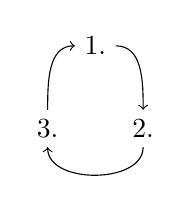
\begin{tikzpicture}[scale=.7]
\node[draw=none] (x) at (0,1) {1.};
\node[draw=none] (y) at (0.866025,-0.5) {2.};
\node[draw=none] (z) at (-0.866025,-0.5) {3.}; 
\draw[->] (x) to[in=90,out=0] (y);
\draw[->] (y) to[in=-90,out=-90] (z);
\draw[->] (z) to[in=180,out=90] (x);
\end{tikzpicture}
\end{center}
\begin{enumerate}
\item[$(1 \implies 2)$] Let $T$ be a linear transformation, 
$a,b \in \mathbb{R}$ and $\vec{v},\vec{w} \in \mathbb{R}^n$. Then
\begin{align*}
T(a\vec{v}+b\vec{w}) &= T(a\vec{v})+T(b\vec{w})\\
&= aT(\vec{v})+bT(\vec{w})
\end{align*}
Since the choice of $a,b \in \mathbb{R}$ and $\vec{v},\vec{w} \in \mathbb{R}^n$
was arbitrary this equality holds for all choices of these values.

\item[$(2 \implies 3)$] Let $T(a\vec{v}+b\vec{w})=aT(\vec{v})+bT(\vec{w})$ for all $a,b \in \mathbb{R}$ and $\vec{v},\vec{w} \in \mathbb{R}^n$. We proceed by mathematical induction on $k$.\\[10pt] 
\begin{inparaenum}
\item[\textbf{Basis Step:}] For $k=1$ let $a_1 \in \mathbb{R}$ and 
$\vec{v}_1 \in \mathbb{R}^n$. Let $\vec{w} \in \mathbb{R}^n$ be any other 
vector. Then 
\begin{align*}
T(a_1\vec{v}_1)&=T(a_1\vec{v}_1+\vec{0})\\
&=T(a_1\vec{v}_1+0\vec{w})\\
&=a_vT(\vec{v}_1)+0T(\vec{w})\\
&=a_vT(\vec{v}_1)+\vec{0}\\
&=a_vT(\vec{v}_1)
\end{align*}

Since the choice of $a_1$ and $\vec{v}_1$ were arbitrary this equality holds 
for all $a_1 \in \mathbb{R}$ and $\vec{v}_1 \in \mathbb{R}^n$.\\[10pt] 
%
\item[\textbf{Induction Hypothesis: }] Suppose 
$T(a_1\vec{v}_1+a_2\vec{v}_2+\cdots+a_k\vec{v}_k)=
a_1T(\vec{v}_1)+a_2T(\vec{v}_2)+\cdots+a_kT(\vec{v}_k)$ for all integers $k$ 
with $1 \le k \le N$. \\[10pt] 
%
\item[\textbf{Induction: }]Let $a_1, \ldots, a_N,a_{N+1} \in \mathbb{R}$ and 
$\vec{v}_1,\ldots,\vec{v}_N,\vec{v}_{N+1} \mathbb{R}^n$. Define 
$\vec{v}=a_1\vec{v}_1+\cdots+a_N\vec{v}_N$. 

Then by the induction hypothesis $T(\vec{v})=a_1T(\vec{v}_1)+\cdots+a_NT(\vec{v}_N)$. Therefore,

\begin{align*}
T(a_1\vec{v}_1+\cdots+a_N\vec{v}_N+a_{N+1}\vec{v}_{N+1})
&=T(1\vec{v}+a_{N+1}\vec{v}_{N+1})\\
&=1T(\vec{v})+a_{N+1}T(\vec{v}_{N+1})\\
&=a_1T(\vec{v}_1)+\cdots+a_NT(\vec{v}_N)+a_{N+1}T(\vec{v}_{N+1})
\end{align*}
Which proves this case by mathematical induction.
\end{inparaenum}

\item[$(3 \implies 1)$] Suppose 
$T(a_1\vec{v}_1+a_2\vec{v}_2+\cdots+a_k\vec{v}_k)=
a_1T(\vec{v}_1)+a_2T(\vec{v}_2)+\cdots+a_kT(\vec{v}_k)$ for all integers $k$ with $k \ge 1$.

Let $r\in \mathbb{R}$ and $\vec{v} \in \mathbb{R}^n$.
Then consider the $k=1$ case $a_1=r$ $\vec{v}_1=\vec{v}$. Then 
\begin{align*}
T(r\vec{v})&=T(a_1\vec{v}_1)\\
&=a_1T(\vec{v}_1)\\
&=rT(\vec{v})
\end{align*}
Therefore $T$ preserves scalar multiplication.

Let $\vec{v},\vec{w} \in \mathbb{R}^2$. Consider the $k=2$ case where we let 
$a_1=a_2=1$, $\vec{v}_1=\vec{v}$ and $\vec{v}_2=\vec{w}$. Then
\begin{align*}
T(\vec{v}+\vec{w})&=T(a_1\vec{v}_1+a_2\vec{v}_2)\\
&=a_1T(\vec{v}_1)+a_2T(\vec{v}_2)\\
&=1T(\vec{v})+1T(\vec{w})\\
&=T(\vec{v})+T(\vec{w})
\end{align*}
Thus $T$ also preserves vector addition and is therefore a 
linear transformation.
\end{enumerate}
\end{proof}

\subsubsection{Exercises}
%\addcontentsline{toc}{subsubsection}{Exercises}


\subsection{The Standard Matrix of a Linear Transformation}
\index{The Standard Matrix of a Linear Transformation}

\begin{definition}
If linear transformation $T:\mathbb{R}^n \to \mathbb{R}^m$ has a matrix 
$A \in M_{m\times n}(\mathbb{R})$ such that $T(\vec{v})=A\vec{v}$ then $A$ 
is called \emph{the standard matrix} of $T$.
\end{definition}

\begin{theorem} Every linear transformation $T:\mathbb{R}^n \to \mathbb{R}^m$ 
has a standard matrix $A=[\vec{a}_1,\vec{a}_2, \ldots, \vec{a}_n]$. In fact,
$\vec{a}_k=T(\vec{e}_k)$ for each integer $k$ with $1 \le k \le n$ 
where $\{\vec{e}_1,\vec{e}_2,\ldots,\vec{e}_n\}$ are the standard basis for 
$\mathbb{R}^n$.\label{thm:standard_matrix}
\end{theorem}

\begin{proof}
It suffices to show that $T(\vec{v})=A\vec{v}$ for all 
$\vec{v} \in \mathbb{R}^n$.
Let $\vec{v} \in \mathbb{R}^n$ be an arbitrary, but fixed, vector. By 
Proposition~\ref{prop:e_k_spans_Rn} $\vec{v}$ is a linear combination of the 
standard basis. In fact, it can be written:
\[
\vec{v}=v_1\vec{e}_1+v_2\vec{e}_2+\cdots+v_n\vec{e}_n
\]

where the each $v_k$ is the $k^{\text{th}}$ coordinate of $\vec{v}$. Thus
\begin{align*}
T(\vec{v}) 
&=T(v_1\vec{e}_1+v_2\vec{e}_2+\cdots+v_n\vec{e}_n)\\
&=v_1T(\vec{e}_1)+v_2T(\vec{e}_2)+\cdots+v_nT(\vec{e}_n)\\
&=v_1\vec{a}_1+v_2\vec{a}_2+\cdots+v_n\vec{a}_n\\
&=[\vec{a}_1,\vec{a}_2,\ldots,\vec{a}_n]
\begin{bmatrix}v_1\\v_2\\\vdots\\v_n\end{bmatrix}\\
&=A\vec{v}
\end{align*}
\end{proof}
